\begin{figure*}[t]
  \centering
  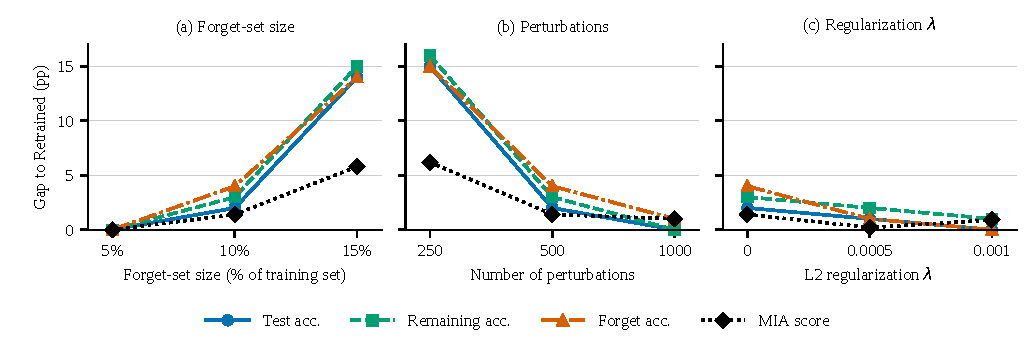
\includegraphics[width=\linewidth]{figures/fig_ablations.pdf}
  \caption{Gap between Unlearned($-$) and Retrained as a function of (a) the forget-set size, (b) the number of perturbations used for Hessian estimation and (c) the L2 regularization $\lambda$ (CIFAR-10, linear classifier). Each curve is the absolute difference in percentage points (pp) for one metric; lower is better and 0 means identical to Retrained. Unless varied, the settings are 10\% forget set, 500 perturbations and $\lambda=0$. Single run per setting; absolute values in \cref{tab:ablations}.}
  \label{fig:ablations}
\end{figure*}
